\hypertarget{point_8h}{
\section{Referencia del Archivo point.h}
\label{point_8h}\index{point.h@{point.h}}
}


\subsection{Descripci\'{o}n detallada}
Implementacion de un objeto punto en 2 dimensiones 

Definici\'{o}n en el archivo \hyperlink{point_8h-source}{point.h}.



Este gr\'{a}fico muestra que archivos directa o indirectamente incluyen a este archivo:\begin{figure}[H]
\begin{center}
\leavevmode
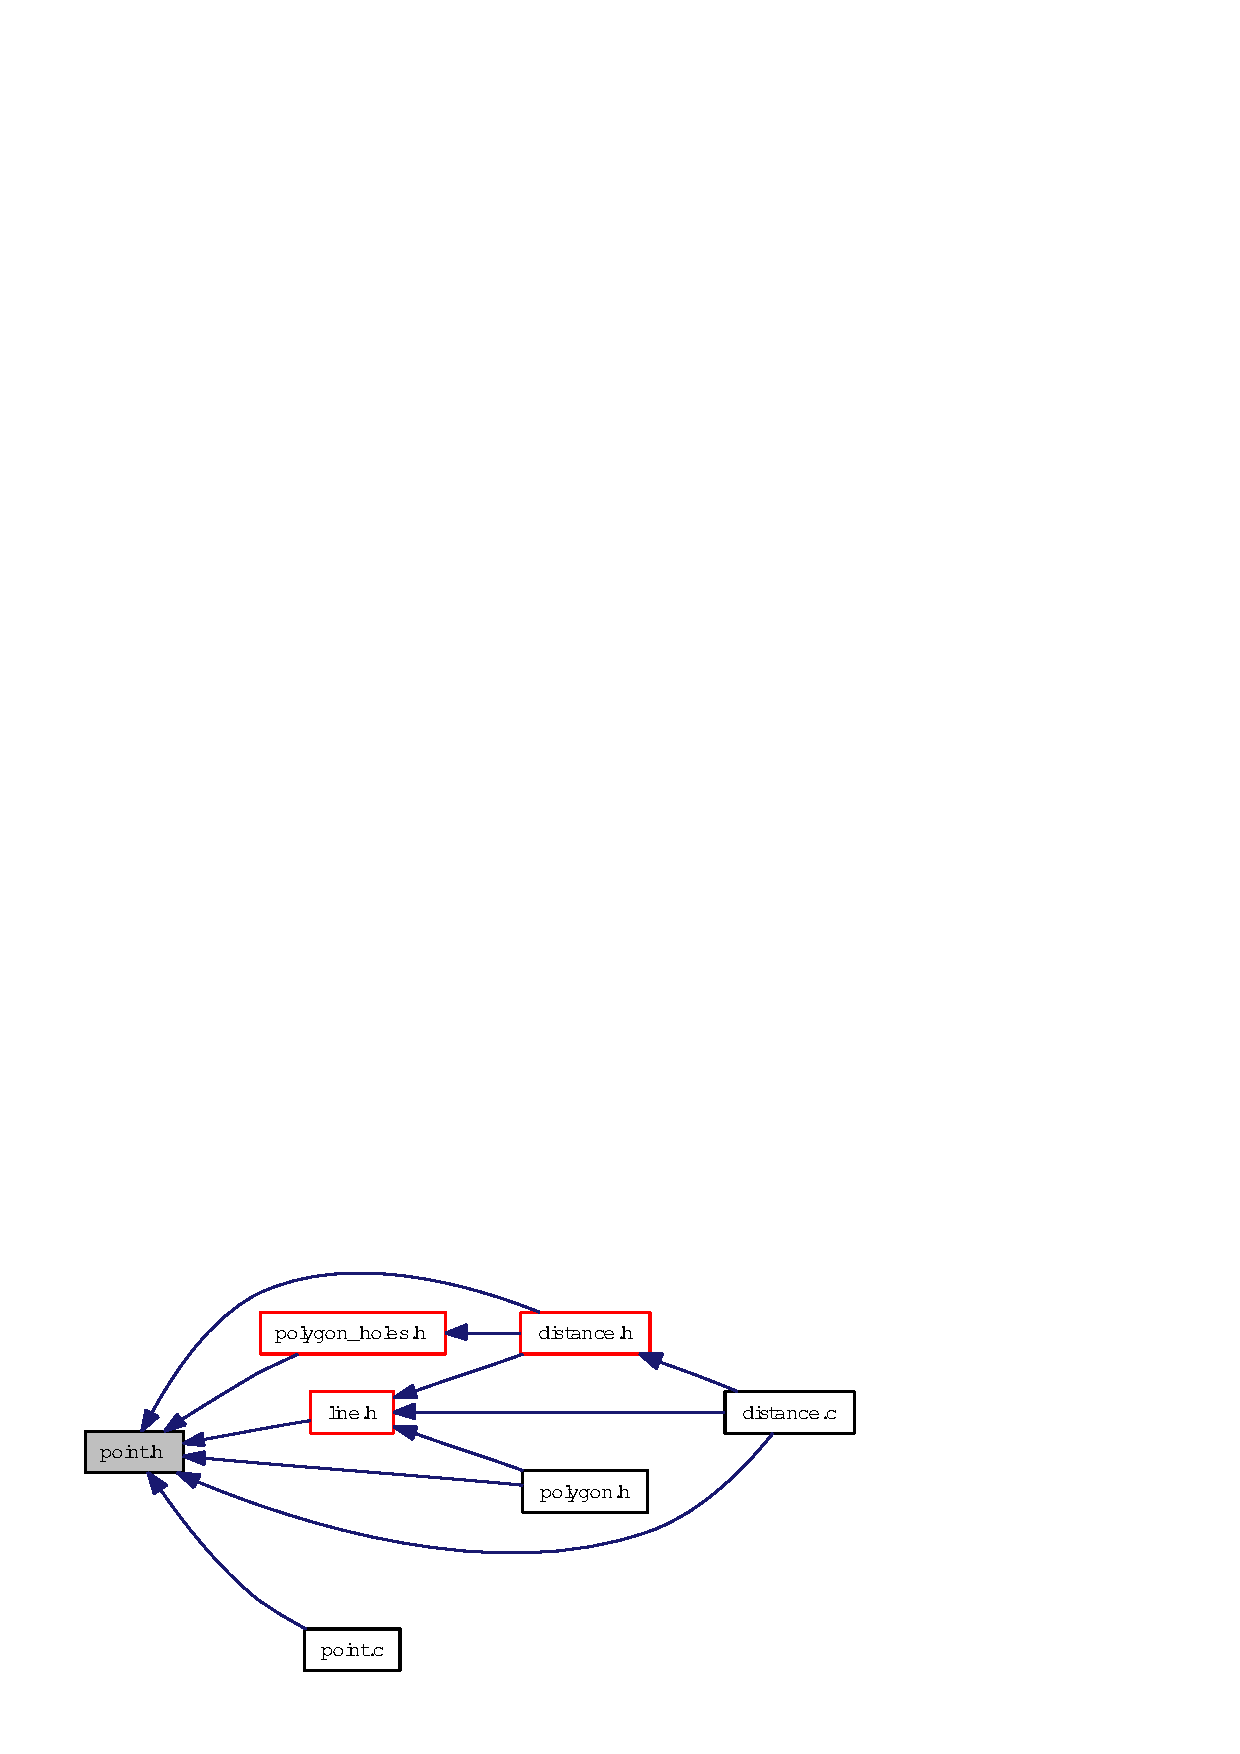
\includegraphics[width=207pt]{point_8h__dep__incl}
\end{center}
\end{figure}
\subsection*{Clases}
\begin{CompactItemize}
\item 
struct \hyperlink{struct__point}{\_\-point}
\end{CompactItemize}
\subsection*{Tipos definidos}
\begin{CompactItemize}
\item 
typedef \hyperlink{struct__point}{\_\-point} \hyperlink{group__geometry_g37e9de632d1eb76ff7dcd3d8172add7d_g37e9de632d1eb76ff7dcd3d8172add7d}{point}
\end{CompactItemize}
\subsection*{Funciones}
\begin{CompactItemize}
\item 
float \hyperlink{group__geometry_ga7ae8d919209fea43e8a61215398bbbe_ga7ae8d919209fea43e8a61215398bbbe}{point\_\-dot} (\hyperlink{struct__point}{point} $\ast$a, \hyperlink{struct__point}{point} $\ast$b, \hyperlink{struct__point}{point} $\ast$c)
\item 
float \hyperlink{group__geometry_gb97527165a510655ee37cd3ccfa8d932_gb97527165a510655ee37cd3ccfa8d932}{point\_\-cross} (\hyperlink{struct__point}{point} $\ast$a, \hyperlink{struct__point}{point} $\ast$b, \hyperlink{struct__point}{point} $\ast$c)
\end{CompactItemize}
